% Intended LaTeX compiler: pdflatex
\documentclass[a4j, 11pt]{jarticle}
\usepackage[dvipdfmx]{graphicx}
\usepackage[dvipdfmx]{color}
\usepackage{indentfirst}
\usepackage{fancyhdr}
\usepackage{lastpage}
\usepackage{amsmath, amssymb, bm}
\usepackage{minted}
\makeatletter
\author{201611350 江畑 拓哉}
\date{2017年10月16日}
\title{演習課題2}

\pagestyle{fancy}

% headers & footers
\lhead{数理アルゴリズム \@title 提出日:\@date\\\@author}
\chead{}
\rhead{}
\lfoot{}
\cfoot{\thepage /\pageref{LastPage}}
\rfoot{}
\renewcommand{\headrulewidth}{0pt}
\renewcommand{\footrulewidth}{0pt}
\makeatother

\begin{document}


\section{課題1}
\label{sec:orgbde3ad9}
\subsection{}
\label{sec:org8425996}
 次に示す配列 a, b からなるデータ列を配列 a の i 番目の要素 a i を横軸に,配列 b の i 番目の要素 b i を縦軸としたグラフを描画せよ.その際, plot 関数を使うこと.\\
\begin{minted}[frame=lines,linenos=true,obeytabs,tabsize=4]{Scilab}
plot(a, b)
\end{minted}


\begin{center}
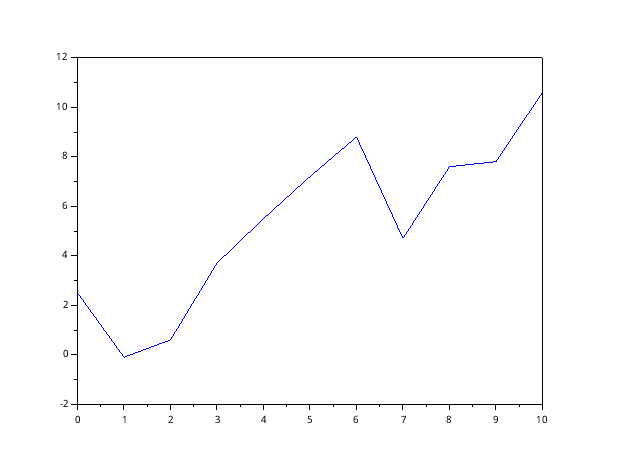
\includegraphics[width=10cm]{./1-1.png}
\end{center}
\subsection{}
\label{sec:org0c8a648}
 (1-1) で用いたデータ列を使用して,破線と任意のマーカーを用いてグラフを描画せよ.\\
\begin{minted}[frame=lines,linenos=true,obeytabs,tabsize=4]{Scilab}
plot(a, b, '--*')
\end{minted}

\begin{center}
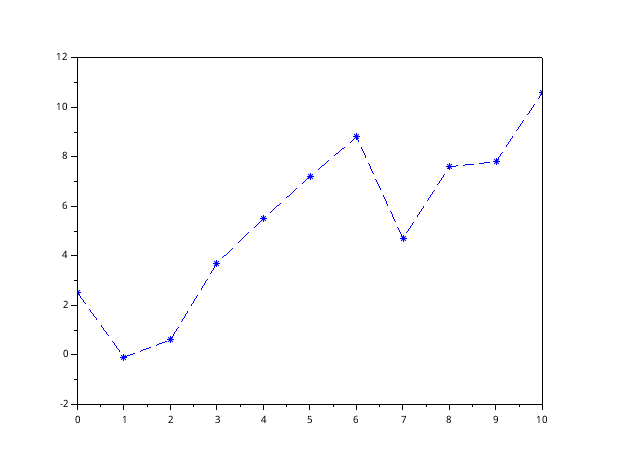
\includegraphics[width=10cm]{./1-2.png}
\end{center}
\subsection{}
\label{sec:org4db939d}
 (1-2) で描画したグラフに対して,タイトルと軸ラベルを表示せよ.\\
\begin{minted}[frame=lines,linenos=true,obeytabs,tabsize=4]{Scilab}
--> plot(a, b, '--*')

--> title('Plot Test')

--> xlabel('ai')

--> ylabel('bi')
\end{minted}

\begin{center}
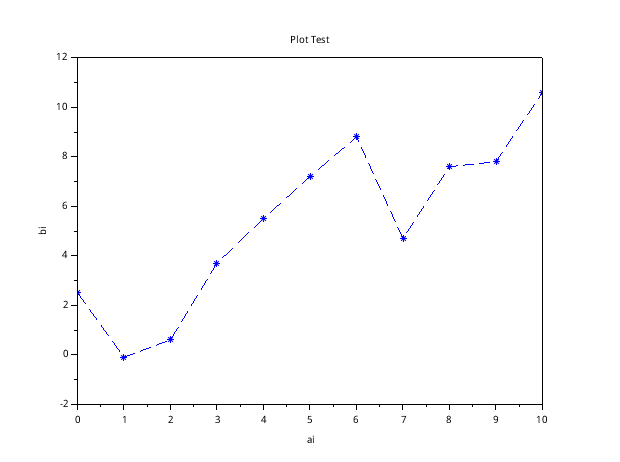
\includegraphics[width=10cm]{./1-3.png}
\end{center}
\section{課題2}
\label{sec:org6071a01}
次に示すベクトルからなるデータ列を片対数グラフで描画せよ.また,通常のグラフも描画し,片対数グラフと比較して違いを考察せよ.\\
\begin{minted}[frame=lines,linenos=true,obeytabs,tabsize=4]{Scilab}
--> a = [0, 1, 2, 3, 4, 5, 6, 7, 8, 9, 10]
--> b = [0.5, 0.6, 1.5, 1.4, 1.3, 360, 180, 160, 130, 200, 80]
--> plot2d('nn', a, b)
\end{minted}

\begin{center}
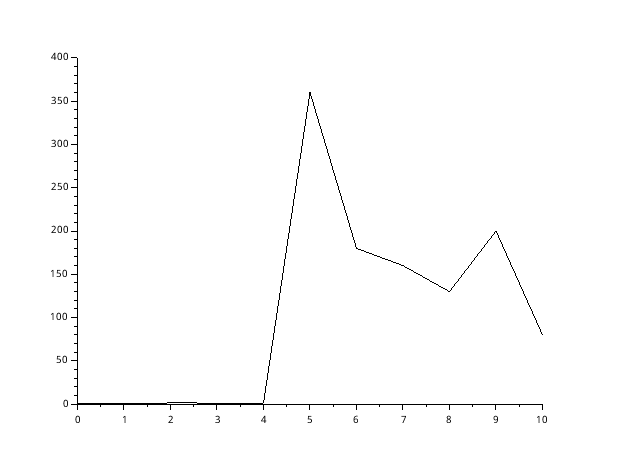
\includegraphics[width=10cm]{./2-no-kata.png}
\end{center}

\begin{minted}[frame=lines,linenos=true,obeytabs,tabsize=4]{Scilab}
--> plot2d('nl', a, b)
\end{minted}
\begin{center}
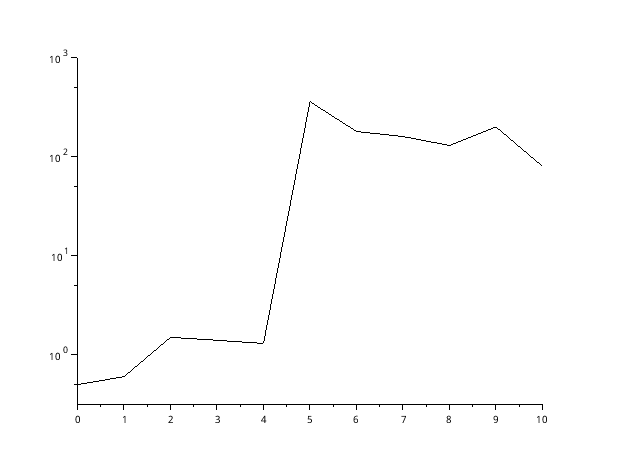
\includegraphics[width=10cm]{./2-kata.png}
\end{center}
 b の値の分布に偏りがある場合、通常のグラフでは変化の小さい部分に対する変化がほとんど視認できないが、片対数グラフにすることによってその変化を視認できるようになる。\\
\section{課題3}
\label{sec:org1a3c2a0}
\(z = e^{x^2+y^2}\) のグラフを surf 関数を用いて描画せよ.\\
\begin{minted}[frame=lines,linenos=true,obeytabs,tabsize=4]{Scilab}
surf(linspace(-0.5, 0.5, 100), linspace(-0.5, 0.5, 100), ..
exp(repmat((linspace(-0.5, 0.5, 100))^2, 100, 1) + ..
(repmat((linspace(-0.5, 0.5, 100))^2, 100, 1))'));
\end{minted}
\begin{center}
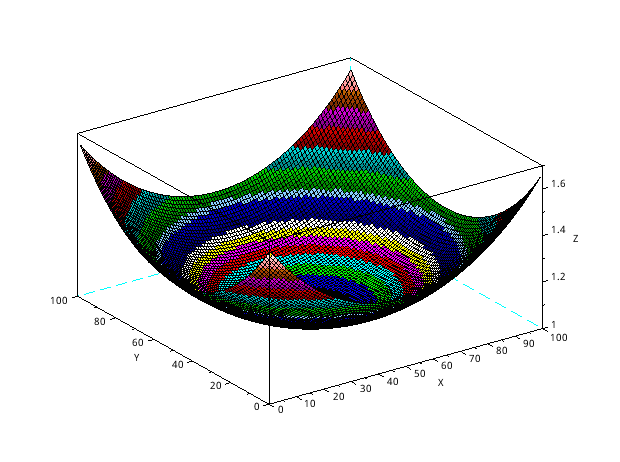
\includegraphics[width=10cm]{./3.png}
\end{center}
\section{課題4}
\label{sec:org4d9470c}
\subsection{}
\label{sec:org7fbc936}
x 軸の範囲,分割点数および係数をパラメータとして多項式関数の描画を行う Scilab の関数を作成せよ.\\
\begin{minted}[frame=lines,linenos=true,obeytabs,tabsize=4]{Scilab}
function [] = createGraph(xfrom, xto, m, a)
x = linspace(xfrom, xto, m);
y = zeros(1, m);
n = size(a, 2) - 1;
for i=1:n
    y = (y + a(i)) .* x;
end
y = y + a(n + 1);
plot(x, y)
endfunction
\end{minted}
\subsection{}
\label{sec:org4512a98}
\(y=-2x^3+x^2+2x+3\) \((-3\leq x\leq 3)\) および\\
\(y = 0.4x^4 - 4.7 x^2 + 4.1x - 4\) \(( -4 \leq x \leq 4)\) のグラフを描画せよ.\\
\begin{minted}[frame=lines,linenos=true,obeytabs,tabsize=4]{Scilab}
--> createGraph(-3, 3, 30, [-2, 1, 2, 3])
--> createGraph(-4, 4, 30, [0.4, 0, -4.7, 4.1, -4])
\end{minted}
\begin{center}
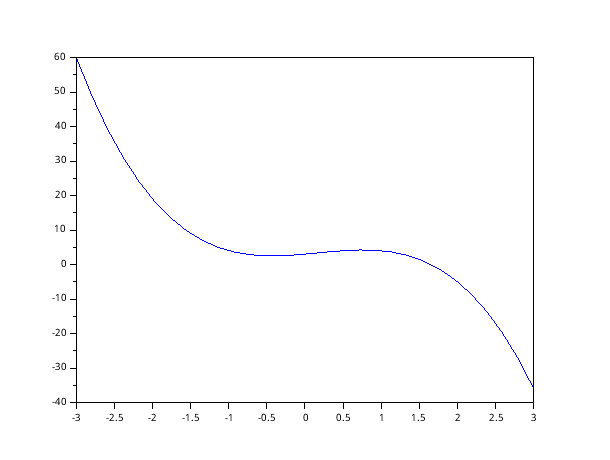
\includegraphics[width=10cm]{./4-1.png}
\end{center}
\begin{center}
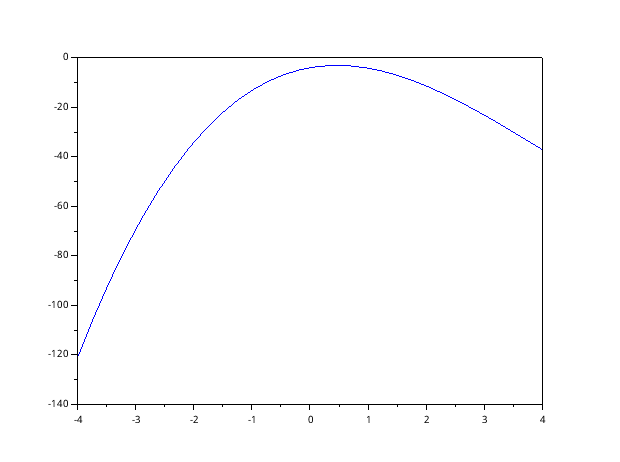
\includegraphics[width=10cm]{./4-2.png}
\end{center}
\end{document}
